\subsection{Aplicação Fábrica: 2ª Via do código de barras}
\subsubsection*{Descrição do caso de uso}
Na obtenção de uma segunda via de um código de barras, espera-se que utilizador entre na página e indique o tipo de código de barras e o código de barras que pretende. 

\begin{figure}[H] 
	\begin{center}
		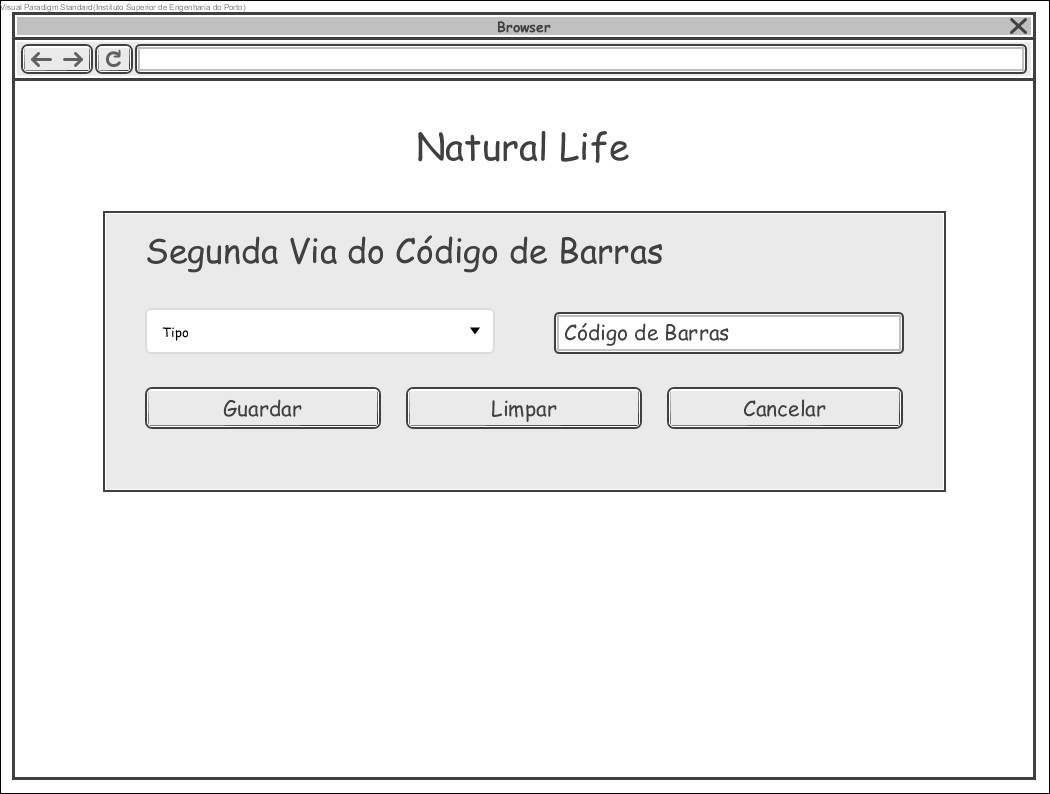
\includegraphics[width=0.60\textwidth,keepaspectratio]{figuras/Diagramas_vp/DI_Fabrica_6_2_Via_Codigo_de_Barras.jpg}
		\caption{Modelo do formulário de pedido de 2ª via de código de barras}
		\label{fig:di_2_via} 
	\end{center}
\end{figure}

\subsubsection*{Fluxo do caso de uso}
O caso de uso inicia-se com a abertura da página do pedido de segunda via de código de barras. É apresentado para o utilizador indicar o tipo de código de barras e o código de barras que pretende. Após indicar as informações solicitadas precisona o botão "Guardar". É aberto um novo separador com o código de barras solicitado para imprimir.

\begin{figure}[H] 
	\begin{center}
		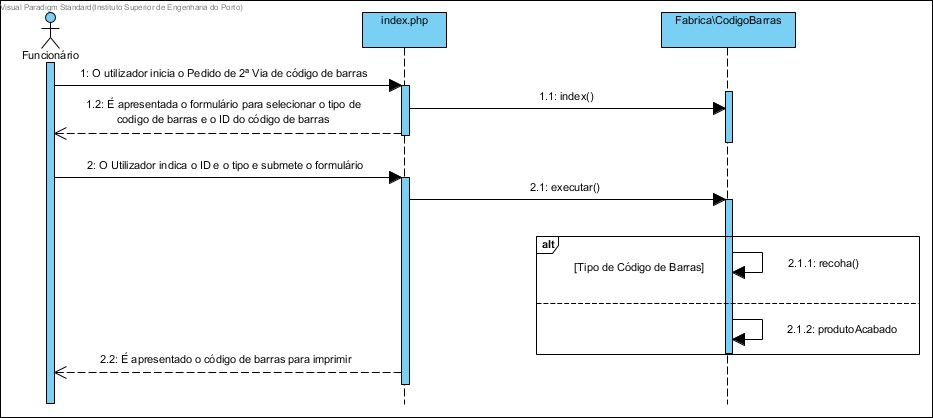
\includegraphics[width=\textwidth,keepaspectratio]{figuras/Diagramas_vp/SD_Fabrica_6_2_Via_Codigo_de_Barras.jpg}
		\caption{Diagrama de sequência de pedido de 2ª via de código de barras}
		\label{fig:sd_2_via} 
	\end{center}
\end{figure}